\documentclass{article} % For LaTeX2e
\usepackage{nips14submit_e,times}
\usepackage{hyperref}
\usepackage{url}
%\documentstyle[nips14submit_09,times,art10]{article} % For LaTeX 2.09

\usepackage{graphicx}

\usepackage{float}
%\usepackage{subfig}
%\usepackage[]{algorithm2e}
%\usepackage{algorithm}
%\usepackage{algorithmic}	
\usepackage{url}%refer to website
\usepackage{caption}
%\usepackage{subcaption}
%\usepackage{subfigure}
\usepackage{color}
\usepackage{algorithm}
\usepackage{algpseudocode}
\usepackage{graphics}
\usepackage{epsfig}
\usepackage{subfigure}
\usepackage{booktabs}
\usepackage{tabularx}
\usepackage{amsmath}


\newcommand{\argmin}{\arg\!\min}
\DeclareMathOperator{\Tr}{Tr}
\bibliographystyle{abbrv}


\title{EECS 545 Project Report: A Review on the Confidence Weighted Mean Reversion Strategy for Online Portfolio Selection}

\def\anticor{{\textsc{Anticor}}}

\author{
Dongyao Chen$\ddagger$, Sihui Han$\ddagger$, Han Lin$\ddagger$, Guangsha Shi$\dagger$\\
Department of Electrical Engineering and Computer Science$\ddagger$\\
Department of Materials Science and Engineering$\dagger$\\
University of Michigan, Ann Arbor, MI-48105, USA\\
\texttt{\{chendy, sihuihan, linhan, guangsha\}@umich.edu}
}

% The \author macro works with any number of authors. There are two commands
% used to separate the names and addresses of multiple authors: \And and \AND.
%
% Using \And between authors leaves it to \LaTeX{} to determine where to break
% the lines. Using \AND forces a linebreak at that point. So, if \LaTeX{}
% puts 3 of 4 authors names on the first line, and the last on the second
% line, try using \AND instead of \And before the third author name.

\newcommand{\fix}{\marginpar{FIX}}
\newcommand{\new}{\marginpar{NEW}}


\nipsfinalcopy % Uncomment for camera-ready version
\graphicspath{{./figures/}}

\begin{document}
\maketitle
\begin{abstract}
This project focuses on the review of the Confidence Weighted Mean Reversion (CWMR) strategy\cite{OnlinePortfolio} proposed by Li \emph{et al.} for online portfolio selection. The CWMR strategy models the portfolio vector as a Gaussian distribution and sequentially updates the distribution (mean and covariance) according to the mean reversion trading idea. We reproduced a cumulative gain of around 10$^{18}$\% after 5600 trading days as was claimed in the paper, and found this astronomical gain was also achievable in different time periods and various stock markets. Finally, we propose a revised method, named ``A-Stock-A-Day Confidence Weighted Mean Reversion" (ASAD-CWMR), which maintains the power of original approach and greatly reduces the transaction cost, and is thus more feasible for personal investments.
\end{abstract} 



\section{Introduction}
Online portfolio selection is a sequential process, which aims to determine a practical strategy for allocating investments among a set of stocks to achieve some financial goals in the long run. Most portfolio selection strategies can be classified into two large groups: trend following and mean reversion. The trend following strategy assumes that historically better-performing stocks would also perform better than others in future. Although this idea is easy to understand, it was found to be violated in short term, for example, if we try to follow the daily trend\cite{JOFI:JOFI5110}.

The mean reversion strategy, on the other hand, believes that if a stock performs worse than others today, it tends to perform better than others in the next trading day. One of the most robust mean reversion methods is the Anticor algorithm proposed by Borodin \emph{et al.}, which obtains a high profit by actively reverting to the mean\cite{AntiCor}.

The CWMR strategy we focus on in the report has an even better performance than Anticor, because it does not only exploit the first order information of the portfolio (mean), but also reflects the second order information (volaility) by constructing the Gaussian distribution of the portfolio vector\cite{OnlinePortfolio}. The key idea of CWMR is to formulate the Gaussian distribution of the portfolio vector that can effectively exploit both its first and second order information and sequentially update this distribution for every trading day. When the portfolio is updated, the CWMR strategy either passively keeps last portfolio, if it had a poor performance in the previous day, or aggressively approaches a new portfolio that would have had an even worse performance in the previous day.

With the CWMR strategy, Li \emph{et al.} reported a cumulative gain of around 10$^{18}$\% after 5600 trading days with a portfolio including 36 NYSE stocks. In this project we implemented the CWMR method and successfully reproduced this astronomical value with the same dataset as they used. To investigate the reliability of CWMR method, we tested it on the up-to-date stock dataset, and found this huge gain was also achievable in different time periods and various stock markets. To better understand the advantage of CWMR method, we also studied and implemented the state-of-art Anticor method for comparison. Finally, we proposed a revised method, named ``A-Stock-A-Day Confidence Weighted Mean Reversion" (ASAD-CWMR), which trades only one stock instead of tens or hundreds of them everyday. ASAD-CWMR method greatly reduces the transaction cost but still maintain the power of mean reversion and guarantee a huge gain in certain periods of time.


\section{Overview}
We consider a financial market with $m$ stocks to invest in for $n$ trading days.  The change of stock prices everyday is represented by a price relative vector $\textbf{x} \in \textbf{R}^m$ with each component denoting the ratio of the closing price to the last closing price of one of the m stocks. A sequence of these price relative vectors $\textbf{x}_1, \cdots, \textbf{x}_n$ describes the price change of the m stocks during n trading days. More specifically, if we invest in the $j$th stock, we will have a reward of $x_{ij}$ on the $i$th trading day.

An investment on the market is specified by a portfolio vector, denoted as $\textbf{b}=(b_1,\cdots,b_m)$, where $b_i$ is the proportion of wealth invested on the $i$th asset. The feasible space of $\textbf{b}$ is denoted by $\Delta_m$, where $\Delta_m =\{\textbf{b}:\textbf{b} \in \textbf{R}^m, \sum_{i=1}^m b_i=1\}$. The investment on the $i$th trading day is defined by a portfolio $\textbf{b}_i$, which increases the wealth by a factor $s_i = \textbf{b}_i^{T}x_i = \sum_{j=1}^m b_{ij}x_{ij}$.  $s_i$ is the portfolio daily return. $\textbf{b}^n$ denotes the portfolio strategy for the $n$ consecutive trading days. Since we re-invest all the wealth, the investment results in multiplicative cumulative return. Thus, after $n$ trading days, the investment of a portfolio strategy $\textbf{b}^n$ produces a portfolio cumulative wealth $\textbf{S}_n$, which is increased by a factor of $\prod_{i=1}^n\textbf{b}_i^T x_i$, i.e., $\textbf{S}_n(\textbf{b}^n,\textbf{x}^n) = \textbf{S}_0\prod_{i=1}^n\textbf{b}_i^T x_i$, where $\textbf{S}_0$ denotes the initial wealth, which is set to \$1 here.

The online portfolio selection problem is a sequential decision task, and we aim to design a strategy to maximize the portfolio cumulative wealth in a sequential fashion. On each trading period $i$, given the historical information, including all the previous sequences of price relative vectors $\textbf{x}^{i-1} =\{x_1 , . . . , x_{i-1} \}$, and the previous sequences of portfolio vectors $\textbf{b}^{i-1} =\{b_1 , \cdots, b_{i-1}\}$, we decide a new portfolio vector $\textbf{b}^i$ for the coming price relative vector $\textbf{x}_i$. This learning and predicting process repeats until the end of the trading period, e.g., $n$ trading days. A portfolio stratergy is evaluated based on the cumulative wealth achieved in the end.

Most portfolio selection strategies, including the methods we will introduce in this report, are based on the three assumptions including (1) no transaction cost; (2) each stock is arbitrarily divisible tradable at its closing price; (3) our investment has no significant impact on the market behavior.

%\subsection{Formulation}



\section{Solution}
The mean reversion method was first proposed by Lo \emph{et al.}\cite{mean_reverse} in 1990. The basic idea is that better performing stocks tend to perform worse than others in the subsequent trading days, and the worse performing stocks are inclined to perform better. Thus to maximize the portfolio return for the next trading day, we can minimize the expected portfolio return with respect to today's price relative since the next price relative tends to revert.  

The CWMR method models the portfolio vector for the $i$th trading day as a Gaussian distribution with mean $\mu\in \textbf{R}^m$ and the diagonal covariance matrix $\Sigma\in \textbf{R}^{m\times m}$ with nonzero diagonal elements $\sigma^2$.  The value $\mu_j$ represents the knowledge of stock $j$ in the portfolio.The diagonal covariance matrix term $\sigma_j^2$ stands for the confidence we have in the portfolio mean value $\mu_j$.  In this case, the authors not only exploit the first order information (mean) of the portfolio, but also combine the second order information of the portfolio (volatility).

Since $\textbf{b}_i \sim \mathcal{N}(\mu, \Sigma)$, and  $\textbf{s}_i = \textbf{b}_i^T x_i$, the daily portfolio return also follows Gaussian distribution: $\textbf{s}_i \sim \mathcal{N}(\mu\cdot x_i, x_i^T\Sigma x_i)$.

If the expected portfolio return using the $i$th price relative is less than a threshold with high probability, the actual return for the $i+1$th trading day tends to be high with correspondingly high probability, since the price relative tends to reverse. Though we are more interested in the stocks with poor performance in the current trading day, we still would like to choose a Gaussian distribution as close to the current distribution $\mathcal{N}(\mu_i,\Sigma_i)$ as possible in the KL divergence sense. Passively choosing the closest distribution alleviates the fluctuation and ensures relatively good performance. On the $i+1$th trading day, the algorithm sets the parameters of the distribution by solving the following optimization problem:

\begin{equation}
\begin{split}
(\mu_{i+1}, \Sigma_{i+1}) &=\argmin_{\mu,\Sigma}~D_{KL}(\mathcal{N}(\mu,\Sigma) || \mathcal{N}(\mu_i,\Sigma_i))\\
& s.t.~ ~\textrm{Pr}[\mu\cdot x_i \le \epsilon] \ge \theta\\
& ~~~~~~~~\mu \in \Delta_m,
\label{eq:orginalOPT}
\end{split}
\end{equation}
The constraint ensures that expected portfolio return using the $i$th price relative is less than a threshold $\epsilon$ with probability larger than $\theta$. $\epsilon$ denotes the mean reversion threshold, and $\theta \in [0,1]$ represents the confidence level of the mean reversion. The constraint intrinsically models the fact that the chosen portfolio has high expectation to have low daily return in current trading day, and potentially has high return in the next trading day.

The combination of the the KL divergence and the constraint follows the idea of Passive Aggressive algorithm\cite{Crammer:2006:OPA:1248547.1248566}. The method is considered aggressive since it may aggressively approach a new portfolio if the constraint condition is no longer fulfilled, i.e., when the current portfolio brings in a high return. On the other hand, it also has a passive character because it will passively keep the current portfolio if the current portfolio keeps having poor performance.

A slight modification is made to the constraint so that it is now convex in covariance: $\epsilon - \log(\mu\cdot x_i) \ge \phi||\Upsilon x_i||$,
where $\Sigma = \Upsilon^2$, $\phi = \Phi^{-1}(\theta)$ and $\Upsilon$ is PSD. The solution to the optimization problem is expressed as:
\begin{equation}
\mu_{i+1} = \mu_{i} - \lambda_{i+1}\Sigma_i\bigg(\frac{x_i-\bar{x}_i\textbf{1}}{\mu_i\cdot x_i}\bigg), ~~~~~~\Sigma_{i+1}^{-1} = \Sigma_i^{-1} + \lambda_{i+1}\phi \frac{x_ix_i^T}{\sqrt{U_i}},
\label{eq:CWMR_update}
\end{equation}
 where $\sqrt{U_i} = \frac{-\lambda_{i+1} V_i\phi+ \sqrt{\lambda_{i+1}^2V_i^2\phi^2 +4V_i} }{2}$ and $V_i = x_i^T\Sigma_ix_i$. $\bar{x_i} = \frac{\textbf{1}^T \Sigma_i x_i}{\textbf{1}^T\Sigma_i \textbf{1}}$ represents the confidence weighted average of the $i$th price relative, and  $\lambda_{i+1}$ denotes the Lagrangian multiplier. Using KKT conditions similar as what we learned in SVM and applying Woodbury equation, we can derive the exact value of $\lambda$.
  
The mean $\mu_1$ and covariance matrix $\Sigma_1$ of portfolio is initialized to be $\frac{1}{m}\textbf{1}$ and $\frac{1}{m^2}\textbf{I}$, correspondingly. Everyday we update the portfolio distribution by updating the mean and covariance matrix according to Eq.~\ref{eq:CWMR_update}. The mean of portfolio is then projected to simplex domain to obtain the required portfolio.

\begin{figure}
%\centering
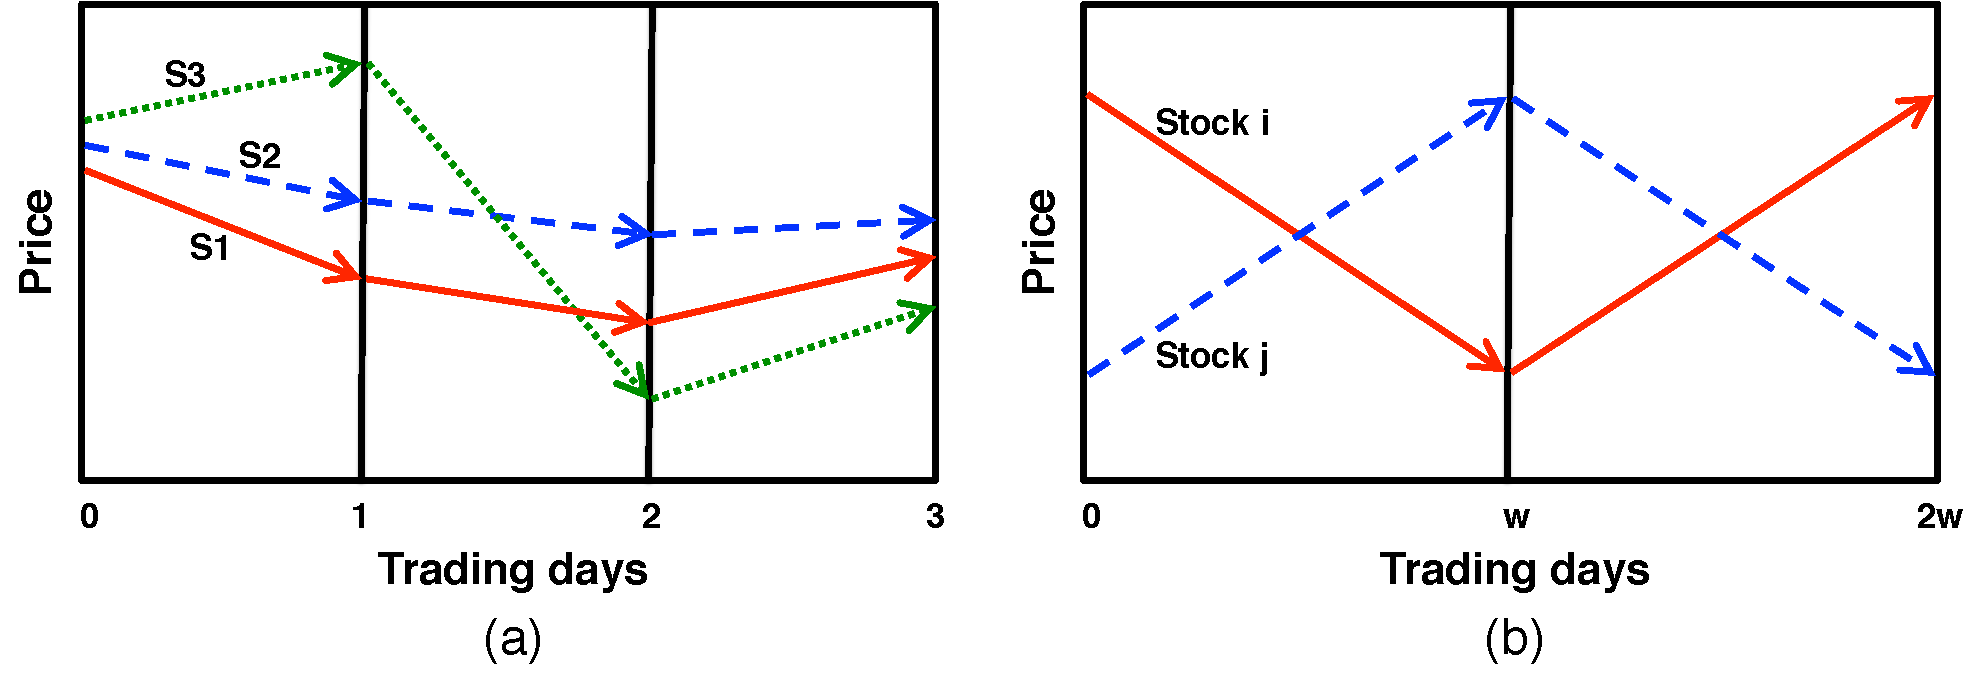
\includegraphics[width=\columnwidth]{illustration}
\caption{
\label{fig:illustration}
Two hypothetical stock charts for the illustration of CWMR and Anticor methods. (a) The price changes of three stocks in three trading days. CWMR assign weights to each stock based on their performance in the current trading day; (b) The price changes of stocks $i$ and $j$ over two consecutive windows with length of $w$ days. Anticor transfers investment from the well-performing stock to the anti-correlated poorly-performing stock.
}
\end{figure}

Let's look at one example on applying CWMR algorithm to three hypothetical stocks S1, S2, and S3 (FIG.~\ref{fig:illustration}(a)). Without any information of the market behavior prior to day 0, we first set the portfolio to be (1/3, 1/3, 1/3), with all the money equally distributed to the three stocks. When it comes to Day 1, we find S1 has the most poor performance so the portfolio may evolve to (1/2, 1/4, 1/4) to fulfill the constraint condition. On Day 2, we notice a big drop of S3, but we do not necessarily have to put more proportion of money on S3 as long as the current portfolio still has a poor performance. Therefore, we may still passively stick to the portfolio of (1/2, 1/4, 1/4). On Day 3, all the stocks rise so there is no way to find a positive portfolio that meet the requirement of the constraint. In that case, we project the calculated portfolio (probably negative) to the simplex domain for a positive portfolio with the smallest return.

The CWMR method does produce a huge return as we will present in the Evaluation section, but it was also pointed out in the paper that the cumulative wealth in the end is very sensitive to the ratio of transaction cost to the money invested. It has been shown that a transaction cost ratio as low as 0.8\% may reduce the final return from $10^{18}$\% to almost zero. This is understandable since CWMR requires trading tens of stocks everyday, and such a large basis of stocks was found necessary to guarantee a considerable amount of return. For this reason, this method may be feasible for large financial institutions, but not for personal investments.

Here we propose a revised method named ``A-Stock-A-Day Confidence Weighted Mean Reversion" (ASAD-CWMR). The idea is we only trade one stock a day though we keep a basis of tens or hundreds of stocks. While we update the portfolio distribution in exactly the same way as in CWMR, we only trade one stock from the portfolio everyday instead of all the stocks with positive components in the portfolio. We select this specific stock by ranking the portfolio components from highest to lowest, and take the first one that has negative performance in the current trading day. It takes much less transaction cost for ASAD-CWMR than for CWMR, and thus make it possible to apply the method even for personal investments. ASAD-CWMR is also more aggressive than the original CWMR method, since it only trades the stock with the highest weight, which is usually (but not always) one of those stocks that have the poorest performance in the current trading day. Every option has its pros and cons. As we will show in the Evaluation section, though ASAD-CWMR leads to higher return in certain periods of time, it has very poor performance during the time when the pattern of mean reversion is not very clear.
 

\section{Related Works}
Besides CWMR, a few other mean-reversion based portfolio selection strategies\cite{UniversalPortfolio, MAFI:MAFI274} have been reported since the idea of mean reversion was first proposed in 1990\cite{mean_reverse}. One of them is the Anticor algorithm introduced by Borodin \emph{et al.} in 2004\cite{AntiCor}.

As we discussed in the previous section, CWMR updates the portfolio for the next trading day by choosing one that has a poor performance today but does not deviate too much from the portfolio used for today. Anticor algorithm has similar characters since it also believes that poor-performing stock is incline to reverse, but it is also very different from CWMR in that Anticor focuses more on the correlations among the stocks.

While CWMR considers the evolution of portfolio as a whole, Anticor applies the mean reversion theory at a much smaller scale, and more specifically, it measures the shift of investment between each pair of stocks every time the portfolio is updated.

The Anticor algorithm evaluates variations in stocks’ performance by dividing a sequence of previous trading days into two periods called windows, with equal length of $w$ days. Anticor tends to transfer investment from stock $i$ to stock $j$ when the following conditions are fulfilled:

1. Stock $i$ had a better performance than stock $j$ over the most recent window.

2. Stock $i$ over the second most recent window is positively correlated with stock $j$ over the most recent window.

3. Both stock $i$ and $j$ are anti-correlated with themselves over consecutive windows.

Figure~\ref{fig:illustration}(b) illustrates a typical case when the investment will be shifted from stock $i$ to $j$. Since the correlation of between stocks $i$ and $j$ in consecutive windows and the anti-correlation of both stocks are supposed to be maintained in the next window, both stocks tend to reverse in the window. Stock $j$, which did not perform well in the most recent window, is predicted to rise in the next window.

For each pair of stocks $i$ and $j$, the extent to which the investment should be shifted from stock $i$ to stock $j$ in the next trading is quantified by $claim_{i\rightarrow j} = M_{cor}(i, j) - M_{cor}(i, i) - M_{cor}(j, j)$ where $M_{cor}(i, j)$ is the correlation between stock $i$ over the second most recent window and stock $j$ over the most recent window, and $M_{cor}(i, i)$ is the correlation between stock $i$ over the second most recent window and itself over the most recent window. Therefore, $claim_{i\rightarrow j}$ will be large if 1) stock $i$ over the second most recent window is positively correlated with stock $j$ over the most recent window and 2) both stock $i$ and $j$ are anti-correlated with themselves over consecutive windows.

As we will show in the Evaluation section, the Anticor algorithm also results in a huge cumulative wealth by constantly transferring investment from the well-performing stock to the anti-correlated poorly-performing stock. The major problem with Anticor is that the return is very sensitive to the window size $w$, the optimal window size may range from 10 days to 50 days depending on which period of time we are interested in.

\section{Evaluation}

We now evaluate the CWMR method, our revised ASAD-CWMR, and Anticor method by performing back tests on real historical data from stock markets. The historical stock data were downloaded from Yahoo Finance. The datasets we used for backtesting are summarized in Table~\ref{tab:dataset}. Datasets NYSE-O and NYSE-N were also used in the previous works\cite{OnlinePortfolio, AntiCor}, while the up-to-date datasets NYSE-5018 and NASDAQ-5018 were collected by us.

\begin{table}
\caption{Summary of 4 real datasets from NYSE and NASDAQ.}
\label{tab:dataset}
\begin{center}
\begin{tabular}{cccc}
\hline
Dataset &  \# Stocks & Time frame &  \# Days \\
\hline
NYSE-O & 36 & July 3, 1962 -- Dec 31, 1984 & 5651 \\
NYSE-N & 23 & Jan 1, 1985 -- June 30, 2010 & 6431 \\
NYSE-5018 & 334 & Jan 1, 1995 -- Dec 5, 2014 & 5018 \\
NASDAQ-5018 & 101 & Jan 1, 1995 -- Dec 5, 2014 & 5018 \\
\hline
\end{tabular}
\end{center}
\end{table}

We set the CWMR parameters $\epsilon$ to -0.5 and $\phi$ to 2, and Anticor window size $w$ to 40. We first successfully reproduced the results of applying CWMR and Anticor on NYSE-O and NYSE-N. In FIG.~\ref{fig:old_data_chart}(a) we present a cumulative return of around $10^{18}$\% after 5600 trading days with 36 NYSE stocks in dataset NYSE-O. The cumulative return with CWMR is around  $10^{15}$ larger than if we simply follows the market. Our ASAD-CWMR method seems to be only slightly better than CWMR, but don't forget that we can save a huge amount of money by reducing the transaction cost. Both CWMR and ASAD-CWMR outperform Anticor, and we believe the reason is the correlation employed in CWMR (current day's performance and next day's performance) is much stronger than the correlation in Anticor (stock behavior in the recent $2w$ days and its performance in the next day). The results on NYSE-N (FIG.~\ref{fig:old_data_chart}(b)) also illustrate the power of CWMR and ASAD-CWMR. We may notice that none of these methods work well after the financial crisis (since the point of 5500 trading days in FIG.~\ref{fig:old_data_chart}(b)).

To further investigate the reliability and stability of CWMR and ASAD-CWMR, we tested them on the up-to-date dataset NYSE-5018 and NASDAQ-5018 which were collected by ourselves. CWMR and ASAD-CWMR did not disappoint us, and still produce an astronomical return of at least $10^{14}$\% in 5018 trading days, or 20 years in both NYSE and NASDAQ markets (FIG.~\ref{fig:long_term_chart}). However, you may notice that the total wealth achieved reaches a peak at a point around 3000 trading days in both NYSE and NASDAQ markets, which is right before the financial crisis. During the financial crisis, the poorly-performing stocks have a large chance to keep their low performance in the next few trading days, and the pattern of mean reversion almost vanishes. Therefore, the application of any mean-reversion based strategy only results in a dramatic loss during the financial crisis. Comparing the returns in the two different markets, we also find that the cumulative return goes up slightly in NASDAQ after the financial crisis, while it does not have a sign of recovery in NYSE. We consider NASDAQ to be a healthier market because NASDAQ has more high-tech companies which are more appealing to investors in recent years.

Nevertheless, we have to admit that now all these mean-reversion methods are not as powerful as they used to be. The financial crisis cast a lingering shadow on people's lives and is still influencing the way people invest their money. However, we believe there should always exist a strong correlation in the stock market. The pattern of mean reversion behavior is just being replaced by another one that requires our further investigation. 

\begin{figure}
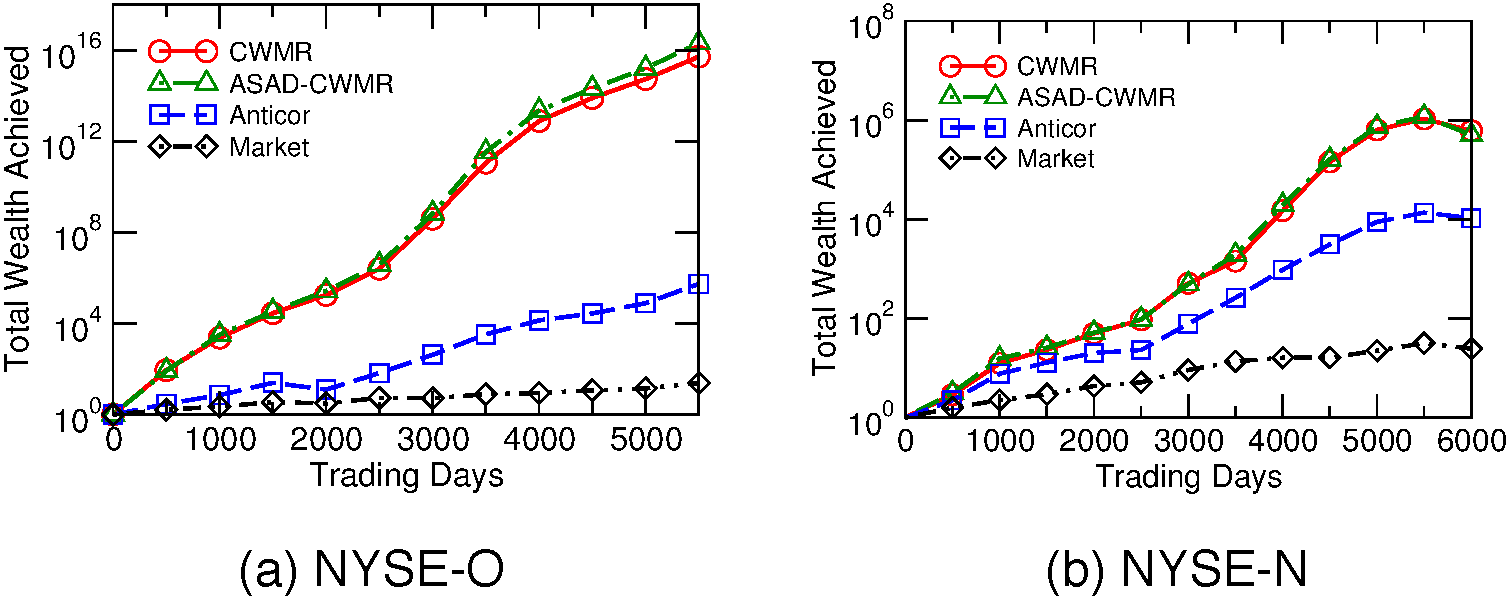
\includegraphics[width=\columnwidth]{old_data_chart}
\caption{
\label{fig:old_data_chart}
Cumulative wealth achieved in dataset (a) NYSE-O and (b) NYSE-N.
}
\end{figure}

\begin{figure}
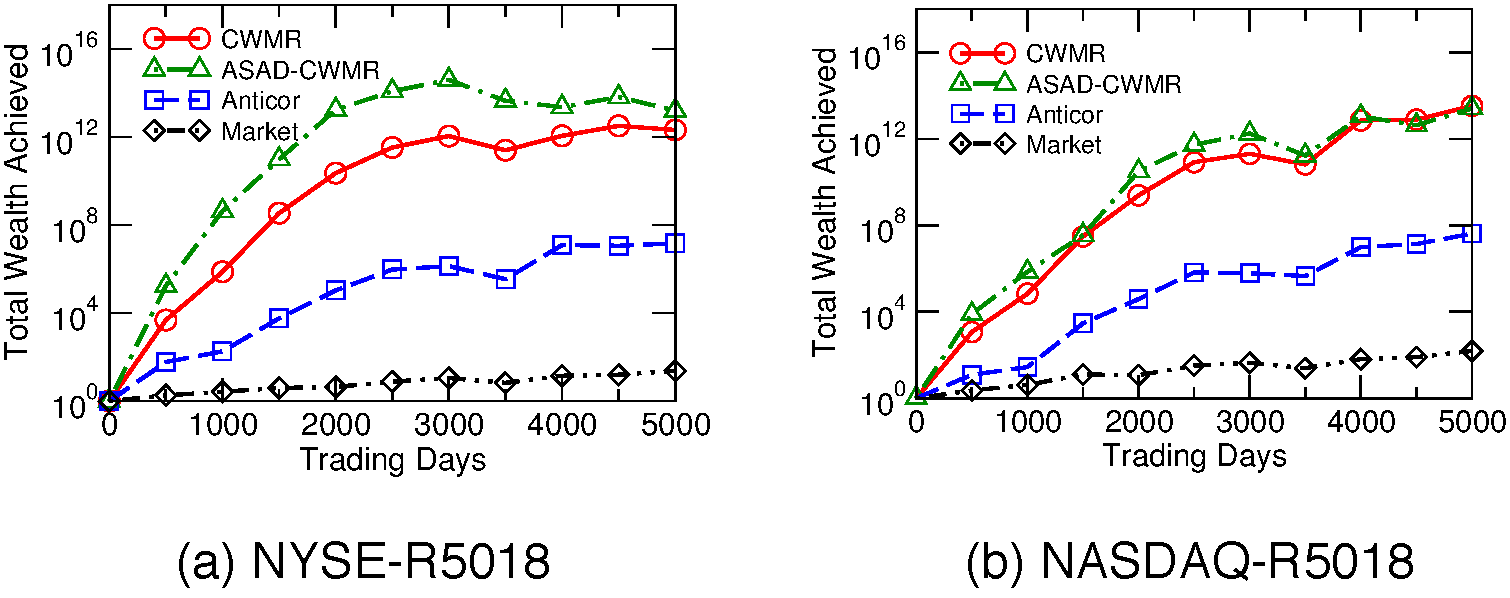
\includegraphics[width=\columnwidth]{long_term_chart}
\caption{
\label{fig:long_term_chart}
Cumulative wealth achieved in dataset (a) NYSE-5018 and (b) NASDAQ-5018.
}
\end{figure}

\section{Conclusion}
In this project we reviewed and implemented the Confidence Weighted Mean Reversion (CWMR) strategy proposed by Li \emph{et al.} for online portfolio selection. We successfully reproduced a cumulative gain of around 10$^{18}$\% after 5600 trading days as was claimed in the paper, and found this astronomical gain was also achievable in different time periods and various stock markets. We also propose a revised method, named ``A-Stock-A-Day Confidence Weighted Mean Reversion" (ASAD-CWMR), which maintains the power of original approach and greatly reduces the transaction cost, and is thus more feasible for personal investments.

Guangsha Shi extracted historical data, designed and backtested the revised ASAD-CWMR algorithm, and evaluated the results. Sihui Han implemented, backtested, and discussed the CWMR algorithm. Han Lin implemented and backtested the Anticor algorithm. Dongyao Chen did an extensive literature review, assessed and discussed the algorithms for comparison.

\small
%\scriptsize
\bibliography{refer}
\normalsize



\end{document}
